\documentclass[11pt,a4paper]{article}
%\usepackage{natbib}
\usepackage[natbib=true, style=authoryear]{biblatex}
\addbibresource{citations.bib}
\usepackage[french]{babel}
\usepackage{textcomp}
\usepackage{csquotes}
\usepackage{setspace}
\usepackage{fancybox}
\usepackage{fancyhdr}
\setlength {\marginparwidth }{2cm}
\usepackage{todonotes}
\usepackage{lipsum}
\usepackage{amsmath}
\usepackage{amsfonts}
\usepackage{amssymb}
\usepackage{pifont}% http://ctan.org/pkg/pifont
\newcommand{\cmark}{\ding{51}}%
\newcommand{\xmark}{\ding{55}}%
\usepackage{bookmark}
\usepackage{mathtools}
\usepackage{scalerel}

\usepackage{diagbox, eqparbox, hhline}
% https://tex.stackexchange.com/questions/150634/how-to-force-a-text-to-appear-after-a-table
\usepackage{placeins}
\usepackage{graphicx}
\usepackage{booktabs}
\usepackage{lscape}
\graphicspath{{Img/}}
\usepackage{float}
\usepackage{titlesec}%remove chapter N
\usepackage{soul} % Texte surligné
\usepackage[left=2cm,right=2cm,top=2cm,bottom=3cm]{geometry}
\setlength{\parindent}{0cm}
\usepackage[framemethod=tikz]{mdframed} %highlight an entire paragraph
\usepackage{framed}
\usepackage{adjustbox}
\usepackage{array}
\usepackage{glossaries}


\usepackage{caption}



\usepackage{comment}


\usepackage{color,soul}
\usepackage{marginnote}
\hypersetup{
    colorlinks,
    citecolor=black,
    filecolor=black,
    linkcolor=black,
    urlcolor=blue
}

\usepackage{listings}
\lstset{
    numbers=left,
    numberstyle=\sffamily\tiny,
    escapeinside={<@}{@>}
}

\usepackage{pdfpages}

\usepackage{hyperref}

\setcounter{secnumdepth}{3}
\setcounter{tocdepth}{3}

\makeatother



\let\labelitemi\labelitemii



\setlength{\doublerulesep}{2.5pt}
\frenchbsetup{ItemLabeli=\textbullet}

\begin{document}
\newcommand{\JMUTitle}[9]{
    \thispagestyle{empty}
    \vspace*{\stretch{1}}
    {\parindent0cm
        \rule{\linewidth}{.7ex}}
    \begin{flushright}
        \vspace*{\stretch{1}}
        \bfseries\Huge
        #1\\
        \vspace*{\stretch{0.2}}
        \bfseries\Large
        #2\\
        \vspace*{\stretch{1}}
        \bfseries\large
        #4\\
        \vspace*{\stretch{1}}
        \bfseries\large
        #9
    \end{flushright}
    \rule{\linewidth}{.7ex}

    \vspace*{\stretch{1}}
    \begin{center}
        \vspace*{\stretch{1}}
        \Large #3 \\

        \vspace*{\stretch{2}}
        \large IFRES. Formasup/CAPAES\\
        \vspace*{\stretch{1}}
        \large   #8 \\[1mm]
        %\vspace*{\stretch{1}}
        \large Année académique: #5 - #6
        %large W{\"u}rzburg, den #6
    \end{center}
}
\JMUTitle
{Plan de cours : Multimédia}                                % Titel der Arbeit
{Développement de jeux vidéos dans un navigateur}                            % Muss in die Kopfzeile passen
{Plan de cours à rédiger dans le cadre du cours PESU0016}       % Art der Arbeit
{Schreurs, Daniel }                              % Vor- und Nachname des Autors
{2022}                                      % Tag der Anemeldung 
{2023}                                      % Tag der Abgabe
{Bachelor/Master Wirtschaftsinformatik}           % Studiengang
{Pascal Detroz, Dominique Verpoorten, Catherine Delfosse et Françoise Jérôme}                       % Name des Betreuers -- Hier sollte *immer* Prof. Winkelmann stehen
{Haute École de la Province de Liège}                                        % Matrikelnummer 
\clearpage
\tableofcontents
\addtocontents{toc}{\protect\thispagestyle{empty}}
\pagenumbering{gobble}


\clearpage
\pagenumbering{arabic}
\section{Informations de base}

\begin{table}[H]
    \begin{tabular}{|l|l|}
        \hline
        Cycle                                        & 1                                  \\ \hline
        Niveau du cadre francophone de certification & 6                                  \\ \hline
        Code                                         & GRA-1-048 2.2.1                    \\ \hline
        Crédits ECTS                                 & 6                                  \\ \hline
        Volume horaire (h/an)                        & 60                                 \\ \hline
        Période                                      & Quadrimestre~2                     \\ \hline
        Implantation(s)                              & TECHNIQUE — Seraing                \\ \hline
        Unité                                        & Orientation                        \\ \hline
        Responsable de la fiche                      & SCHREURS Daniel                    \\ \hline
        Pondération                                  & 60                                 \\ \hline
        Composition de l'unité d'enseignement        & Mutimédia — TP                     \\ \hline
        Prérequis                                    & /                                  \\ \hline
        Corequis                                     & Développement Côté Client (DCC)    \\ \hline
        Intervenants                                 & Maître-assistant~: SCHREURS Daniel \\ \hline
        Contact                                      & {\ul daniel.schreurs@hepl.be}      \\ \hline
    \end{tabular}
\end{table}

\section{Description du cours}

Pourquoi ce cours est-il pertinent ? Parce qu'il vous prépare à votre futur métier. Si vous suivez ce cours, c'est que vous vous destinez à devenir un technicien du web. Que vous soyez plutôt orienté programmation ou conception d'interfaces vous devez avoir de solides compétences en JavaScript puisque soit vous allez concevoir des interfaces graphiques dans quel cas vous devez comprendre comment cela fonctionne et dans l'autre cas vous allez le programmer. Il y aura de l'authenticité et du défi, mais cela restera réalisable parce que justement ce sera très progressif.


Un site internet, s’il n’était composé que d’images et de textes, apparaitrait très statique. On peut grâce à JavaScript le rendre dynamique en faisant réagir son contenu à des évènements que l’utilisateur émet. Par exemple, le clic et le déplacement de sa souris, l’utilisation de son clavier, etc. Les sites internet les plus dynamiques sont les jeux qu’on peut directement jouer dans un navigateur puisqu'il n'y a là plus que des images qui s’animent et qui réagissent à des évènements.
Dans ce cours, nous explorons différentes techniques qui permettent de rendre interactifs les sites internet jusqu’à devenir des jeux. Tout particulièrement en étudiant les possibilités offertes par l’\href{https://developer.mozilla.org/fr/docs/Web/API/Canvas_API}{API canvas}\footnote{https://developer.mozilla.org/fr/docs/Web/API/Canvas\_API} qui est l'interface  de programmation de dessin nativement disponible dans les navigateurs.

Nous commencerons avec des animations 2D simples jusqu’à la réalisation de jeux 2D plus complexes. En revanche, nous n’aborderons pas les concepts 3D.

Ce cours s’inscrit dans la continuité du cours de «~Développement Côté Client (DCC)~», qui a pour but de poser les bases de la programmation côté client avec JavaScript. En troisième année, dans le cadre du cours de «~Développement d'Applications Mobiles (DAM)~», nous aurons régulièrement l’occasion de revenir sur certains concepts étudiés dans ce cours.
\clearpage
\section{Ma philosophie de l’apprentissage}

La première langue que j'ai apprise (et que je parle à la maison), c'est l'allemand. Je n'ai donc pas toujours eu une scolarité aisée. Si aujourd'hui je suis passé outre cette difficulté et que je suis même passé de l'autre côté du banc c'est aussi parce que j'ai eu la chance de rencontrer, durant mon parcours, des enseignants qui ont cru en moi et qui ont su me motiver. Je souhaite donc, à mon tour, aussi donner une chance au plus grand nombre.

Quand je donne cours, j’essaye que chacun ressente le caractère atteignable du cours, particulièrement au début. Par exemple, je prends beaucoup de plaisir, à présenter les projets de vos prédécesseurs, je le fais, car il s’agit là d’une preuve que d’autres y parviennent. Et donc… pourquoi pas vous ? De plus, je fais systématiquement, en début de quadrimestre par cours, un petit test formatif. Je souhaite ainsi identifier ce que vous maitrisez déjà en vue d’adapter les cours en fonction de vos acquis. Cela me permet aussi de vous rediriger, au besoin, vers d'autres ressources spécifiques de manière individuelle. Enfin, j'organise la matière en plaçant stratégiquement la difficulté de sorte qu'elle soit accessible au plus grand nombre le plus longtemps possible. Le tout dans un contexte plutôt libre et autonome afin d'installer un climat de classe motivant tout en évitant la carotte et le bâton. Je cherche plutôt à vous challenger sur des nouveaux défis.

Même si les concepts sous-jacents restent valables, les technologies que j'ai étudiées au début de mon parcours supérieur sont aujourd'hui obsolètes. Non pas parce qu'on m'a enseigné des outils obsolètes, mais parce que l'évolution des nouvelles technologies, dans le domaine de l'information, est à ce point rapide. En 5 ans à peine, il peut y avoir des évolutions significatives. J’essaye donc de répondre à cette réalité en favorisant votre autonomie. Je cherche à vous donner les clés pour comprendre les textes techniques qui vous permettront d’aborder d’autres nouvelles technologies. Il s’agira donc beaucoup «~d’apprendre à apprendre~». Nous aurons régulièrement l’occasion d’analyser des problèmes et d’y apporter des solutions concrètes individuellement ou collectivement. J’utilise donc l'exploration pour introduire les nouveaux concepts et l’apprentissage par projets pour consolider vos connaissances. Je privilégie les activités d’apprentissage\footnote{J'encourage la prise de parole en classe, en veillant à ce que chacun se sentent en sécurité et à l'aise.} en petits groupes (moins de 20) afin de favoriser votre participation et votre sentiment d’inclusion. J’essaye ainsi de vous donner un cadre moins intimidant.


Enfin j'offre un soutien et une ouverture aux élèves qui se sentent marginalisés ou discriminés, en leur offrant un espace sécuritaire et en leur proposant des ressources pour obtenir de l'aide et de l'assistance.

\clearpage
\section{Prérequis et corequis}
\todo{Et c'est moi qui donne le cours}
Ce cours s’inscrit dans la continuité du cours de «~Développement Côté Client~», qui se donne au premier quadrimestre. Ce dernier vous a permis d’acquérir les bases de la programmation côté client, en JavaScript. Nous allons maintenant nous servir de ces acquis pour construire des interfaces multimédias riches. Le cours de «~Développement Côté Client~» devient ainsi le corequis de ce cours.
Si vous n’avez pas acquis les bases ou que vous éprouvez des difficultés en JavaScript, je vous encourage d’une part à refaire les exercices du cours\footnote{Je vous rappelle que les correctifs des exercices sont également disponibles depuis la branche «~complete~».} avec les vidéos explicatives de la chaine «~\href{https://www.youtube.com/@coursdeweb}{coursdeweb}~»\footnote{https://www.youtube.com/\@coursdeweb}. D’autre part à suivre la petite formation en ligne «~\href{https://javascript30.com}{JavaScript30}~»\footnote{https://javascript30.com} de \href{https://wesbos.com}{Wes Bos}\footnote{https://wesbos.com}. J'organise, à la première séance de cours, un test formatif qui vous permet de mesurer votre niveau de maitrise en JavaScript. Dans tous les cas, je reviendrai \underline{individuellement} vers vous.

\begin{figure}[H]
    \begin{center}
        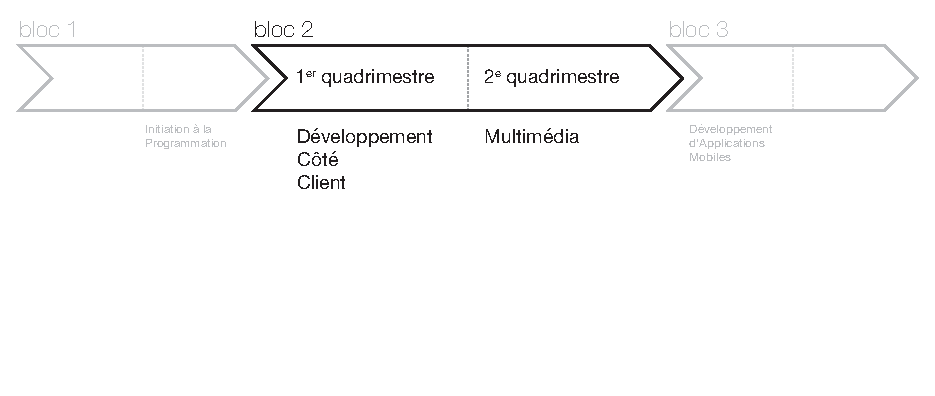
\includegraphics[width=\textwidth]{figures/corequis.eps}
        \caption{Illustration du corequis}
        \label{Fig:GQM}
    \end{center}
\end{figure}
\clearpage

\section{Contenus}
\label{Contenus}
Voici dans l'ordre les différents thèmes que nous aborderons ensemble en classe.
\begin{comment}
Je les classe par catégories, celles-ci sont différentes parties nécessaires à la réalisation d'un jeu. J'aime bien l'analogie de la maison. Avec comme fondations vos compétences en JavaScript et par-dessus les différentes briques/outils nécessaires pour aboutir à quelque chose de complet.
\end{comment}
\begin{enumerate}
    \item Test formatif en JavaScript.
    \item Correction et rappels des concepts de base JavaScript utilisés dans le cadre de ce cours.
    \item Utilisation d’un framework pour compiler les fichiers sources.
    \item Réalisation d'animations 2D simples avec JavaScript.
    \item Réalisation d’un outil qui permet de générer un logo à partir de paramètres encodé par l’utilisateur.
    \item Introduction à l’API de Canvas.
    \item Révision de quelques concepts mathématiques essentiels pour animer des formes. (Radian, degré, périmètres, Sin, Cos, etc.)
    \item Mise en place d’une boucle d’animation. Déplacer aléatoirement et à vitesse constante, des formes dans un canvas.
    \item Déplacer plusieurs formes avec la détection du survol de la souris.
    \item Détecter et interagir avec les évènements émis par l'utilisateur. Clic, survol, clavier, etc..
    \item Utilisez l’API Canvas pour appliquer des traitements sur des images bitmap.
    \item Déplacer des formes avec des images dans un canvas.
    \item Simuler de la neige, de la pluie sous l'effet du vent.
    \item Dessiner et animer le décor d’un jeu 2D avec une sprite sheet.
    \item Réalisation d’un premier jeu complet Flappybird.
    \item Réalisation d’un deuxième jeu complet Asteroids.
    \item Réalisation d’un examen formatif des années précédentes.
    \item Correction de l'examen formatif.
\end{enumerate}
\begin{comment}
\begin{figure}[H]
    \begin{center}
        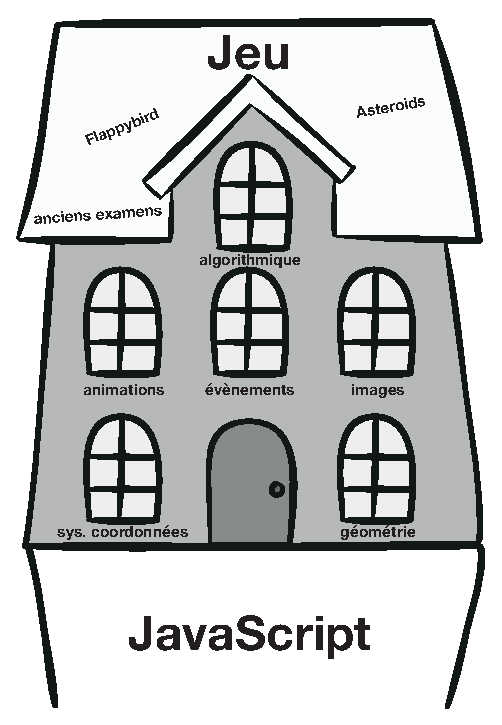
\includegraphics[width=0.3\textwidth]{figures/plan-de-cours.eps}
    \end{center}
\end{figure}
\clearpage
\end{comment}

\subsection{Justifications}

J'ai cherché à calibrer la matière. Au début, les exercices sont plus simples et demandent moins de stratégies cognitives. On pourrait prendre comme mesure quantitative par exemple le nombre de lignes de codes qu'ils doivent produire au fur et à mesure
des exercices. Plus nous avançons dans la matière et plus elles s’empilent. La complexité augmente. Mon objectif étant de maintenir ce sentiment de compétences\cite{viau1994motivation} chez les apprenants.

\clearpage
\section{Visées d’apprentissage}
\begin{itemize}
    \item Savoir programmer des interfaces multimédias riches dans un navigateur.
\end{itemize}

Nous nous limiterons, dans ce cours, aux jeux interactifs à 2~dimensions\footnote{Les jeux interactifs à 2 dimensions sont par essence des interfaces multimédias riches.} en utilisant conjointement l’API de dessin canvas et les bases du langage JavaScript.

\section{Méthodes d’enseignement et activités d’apprentissage}
% Attention : ici il ne faut pas parler... trop pédagogique... 
Vous avez choisi un bachelier professionnalisant, qui cherche donc à vous préparer, au mieux, au mode professionnel. C’est  pourquoi j’ai choisi d’articuler le développement de vos compétences autour de cas réels issu du jeu vidéo. J'utilise la méthode des évènements d’apprentissage\cite{Leclercqevenements} et l'apprentissage par projets\cite{proulx2004apprentissage}.
Le cours se donne au deuxième quadrimestre, une fois par semaine à raison de 4~heures. Voici les types d'activités dominantes.
\begin{enumerate}
    \item Il y aura des moments d'échange. Je m'engage à organiser... vous vocaliser sur la matière... mettre en lumière l'essentiel...Mais vous... vous devez participer... j'ai besoin de votre particulièrement.\todo{TBD}
    \item Étaler les contenus. Space practices... Répéter les choses....C'est toujours les mêmes choses qu'on répéte.(Ici un des 3 points qu'ils proposent c'est justement d'étaler... https://journals.sagepub.com/doi/pdf/10.3102/0013189X10374770)\todo{TBD}
    \item Un prof compétent doit aussi maitriser la technologies....\todo{TBD}
    \item Combiner les super pouvoir des techniques et des avancé pédagogique. Pratiquer un hybride bien pensé.\todo{TBD}
    \item Développer des solutions algorithmiques, dans une forme d’autonomie individuelle ou collective, avec vos connaissances ou en allant chercher d’autres:\\Ceci sur base d’un problème authentique issu du monde du jeu vidéo. Par exemple, comment détecter la collision de 2~formes dans un plan à 2~dimensions ? Ces solutions algorithmiques évolueront jusqu'à devenir des jeux pleinement fonctionnels depuis un navigateur.
    \item Compréhension d'éléments théoriques nécessaires à la réalisation des jeux:\\Parfois «~après l’exercice~» dans quel cas l’activité s’apparente plutôt à de l’exploration. Et d’autres fois «~avant l’exercice~» dans quel cas l’activité s’apparente plutôt à de l’exercisation. Au fil des semaines, vous travaillerez de plus en plus en autonomies étant donné que vos connaissances augmenteront.
    \item Exercisation sur des points de matière concrets:\\Ces exercices couvrent progressivement la matière du cours. Ces derniers sont à réaliser en pleine autonomie chez vous ou en classe. Certains exercices feront l'objet d'une correction collective en classe. Dans tous les cas, toutes les solutions seront disponibles.
    \item Création, à domicile et individuellement, durant les différentes semaines de cours d’un jeu:\\Vous choisissez ce jeu parmi le \href{https://fr.wikipedia.org/wiki/Liste_de_jeux_Atari_2600}{catalogue Atari}\footnote{Ce catalogue comporte 2600 jeux.(https://fr.wikipedia.org/wiki/Liste\_de\_jeux\_Atari\_2600)}. Il s’agit là d’une occasion de vous entrainer à l’examen et de revoir les points de matière du cours. Je vous encourage, au fur et à mesure que nous voyons les concepts théoriques, de les mettre en pratique dans votre jeu.
\end{enumerate}
\subsection{Les techniques}
\begin{itemize}
    \item Advance Organizer, structurant préalable
    \item Perdre du temps à redire ce qui a déjà été dit.
\end{itemize}



\clearpage
\subsection{Justifications}
\begin{itemize}
    \item Transmission/réception : oui et elle est inévitable. Marcel gauchet. conditions de l'éducation....
    \item Le prof activateur... hatties. Quand le prof devient un apprenant et quand l'étudiant devient le prof de son enseignement !!! John Hattie\todo{TBD}
    \item Quelle est ma valeur ajouté de donner mes cours en présentiel ?\todo{TBD}
    \item Etablir des connexion entre les choses...\todo{TBD}
    \item Parler des autres facteurs qui influences la dynamique motivationnelle de l'étudiant...\todo{TBD}
    \item Étant donné que la motivation fait partie de ma philosophie et que l’un des ingrédients de la motivation c’est d’apporter de la valeur aux connaissances\cite{viau1994motivation}, l’approche par projets me permet de rendre concrets mes enseignements au travers de besoins issus de situations authentiques. Concrètement, j'articule la matière autour de besoins afin de faire ressentir l'intérêt des connaissances. Régulièrement, quand la plupart des apprenants ont trouvé une solution, je demande à certains de présenter leur solution de sorte à introduire dans un troisième temps la théorique.  C’est l’occasion de débattre de la matière, mais aussi de susciter leur intérêt pour celle-ci puisqu’ils ont un besoin, résoudre le problème posé au début.
    \item L'évènement d'exploration que je mets en place, quand ils doivent trouver la solution, vise aussi à développer leur autonomie sans pour autant les submerger, avec un problème\footnote{On pourrait considérer ceci comme un apprentissage par problèmes. Cependant, ces problèmes ne sont pas suffisamment centraux, authentiques et complexes pour considérer qu’il s’agit d’un apprentissage par problèmes.} trop compliqué. Dans la première activité, le problème reste simple. En revanche pour l'activité «~projet~» l’autonomie est encore plus forte. Avec un problème plus authentique et compliqué. Nous basculons vers un apprentissage par projets.
    \item «~Make learning visible~» \footnote{The ‘visible’ aspect also refers to making teaching visible to the student, such that they learn to become their own teachers.}\cite{hattie2012visible}. Le projet est aussi une occasion, pour les apprenants (et moi-même), de se rendre compte des savoirs qu'ils acquièrent. Ils voient bien qu'au fur et à mesure que la matière est vue, qu’ils peuvent avancer dans la réalisation de leur propre jeu.
    \item \citet{perrenoud1992differenciation} dit «~différencier, c’est organiser les interactions et les activités de sorte que chaque élève soit constamment ou du moins très souvent confronté aux situations didactiques les plus fécondes pour lui~». J’essaye donc, face à la diversité mathétique, d’apporter une polyvalence didactique. J'applique de manière signifiante l'exercisation, l'exploration, la création et la réception.
    \item Le projet donne aussi un sentiment de contrôle. Ils sont libres d'organiser leur temps pour le projet.
    \item J'accorde une grande importance à la correction des exercices. Cela me semble encore plus important que l'exercice. En début de séance, je demande aux apprenants s'ils souhaitent que je corrige, avec eux, un exercice qui leur semble particulièrement difficile. S’ils n’ont pas de souhaits particuliers, je corrige quand même un exercice pour vérifier la compréhension. C'est une occasion pour eux d’avoir du feedback.
\end{itemize}
\begin{figure}[H]
    \begin{center}
        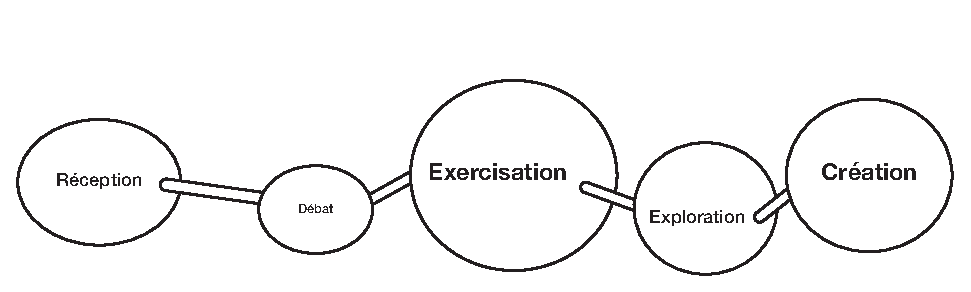
\includegraphics[width=0.8\textwidth]{figures/EAEs.eps}
        \caption{Représentation atomique des évènements dominants \cite{leclercq2008modele}}
    \end{center}
\end{figure}
\clearpage

\section{Évaluation des apprentissages}

\subsection{L’évaluation formative}
\label{eval_formative}

Ces 2 évaluations formatives ont pour but de vous entrainer. De vous offrir une situation authentique supplémentaire pour vous exercer sans pour autant vous pénaliser. Ce qui m'importe ici, c'est que vous appreniez.
\begin{enumerate}
    \item Lors de la première séance~: vous réaliserez un test formatif d’application pratique sur la matière du cours de «~Développement Côté Client~» qui est le corequis de ce cours. Ceci est une occasion pour vous et moi de mesurer votre maitrise en JavaScript.
    \item Lors de l'avant-dernière séance de cours~: vous réaliserez individuellement un examen des années précédentes en classe. Nous consacrerons la dernière séance à sa correction collective où chacun corrige individuellement sa copie d'examen.
\end{enumerate}

\subsection{L’évaluation certificative}
\label{eval_certificative}
L’évaluation certificative s'organise en 2~temps~:
\begin{enumerate}
    \item Vous devez rendre, le jour de l'examen, votre projet de jeu personnel que vous aurez développé individuellement chez vous pendant les différentes semaines de cours. Les consignes vous seront communiquées au premier cours. Vous devez donc gérer votre temps pour ce projet qui compte pour 20~\% de la cote finale.
    \item L'examen pratique consiste à programmer un jeu à partir d'un énoncé\footnote{Je vous rappelle que les énoncés des années précédentes sont disponibles sur l'\href{https://github.com/tecg-mmi}{organisation GitHub} officielle du cours. (https://github.com/tecg-mmi)} qui vous sera fourni et que vous découvrirez le jour même. Vous aurez à votre disposition toutes les ressources du cours, un accès complet aux documentations officielles, ainsi que vos propres productions. Vous disposez de 4~heures pour réaliser cet examen en classe. Ce travail compte pour 80~\% de la cote finale.
\end{enumerate}
Lors de la première séance de cours, je vous présenterai l'énoncé du dernier examen avec sa grille d'évaluation. Elle se construit toujours de la même manière. J'attribue aux fonctionnalités du jeu un degré de complexité. Ensuite, je mesure l'aboutissement des différentes fonctionnalités dans votre proposition. Ces fonctionnalités sont clairement mentionnées dans l'énoncé de l'examen et sont classées par ordre de complexité. Le nombre de points maximum attribué à chaque fonctionnalité est également mentionné.


\subsection{Justifications}
\label{evaluation_des_apprentissages_justifications}
\begin{itemize}
    \item Parler de la motivation intrinsèque. On ne travaille pas que pour des points. On travaille aussi pour soi.\todo{text}
    \item «~L’émission de feedbacks est souvent considérée comme un élément clé pour renforcer la motivation et soutenir la réussite des élèves.~»\cite{georges2011feedbacks}. La réalisation de l'examen formatif est une activité intégrée qui permet de recevoir du feedback. D'une part, sur sa compréhension de la matière, donc plutôt un feedback simple de type assertif et évaluatif\cite{georges2011feedbacks} sur sa performance. D'autre part un feedback plus complexe relatif aux stratégies qu'il faut adaptées (Métacognition). Par exemple, quelles sont les parties plutôt simples et comment rapidement les valider. Ou encore, réfléchir aux éléments plus compliqués, que mes apprenants aiment appeler des «~pièges~»\footnote{Je n'adhère évidemment pas à cette appellation. Mon examen ne contient pas de «~pièges~» sans quoi on pourrait se poser des questions sur mes intentions. L'examen contient des parties plus compliquées qui nécessitent une certaine forme d'inhibition cognitive.}. \citet{hattie2008visible} explique dans son ouvrage que le feedback a un impact significatif sur la performance de l'apprenant. Enfin, c'est une occasion pour entrainer la méta-cognission\cite{leclercq2008modele}. Nous réfléchissons ensemble aux stratégies qu'il faut mettre en place pour réussir l'examen. D'ailleurs chaque année je désigne un «~sécrétaire~» pour cette séance. Il aura pour mission de prendre note de toutes les astuces que nous avons déterminées ensemble afin que les apprenants puissent consulter cette ressource plus tard. D'autre part, je prends soin, dans la rédaction de l'énoncé, d'être constant. À vrai dire, je réutilise un template de base pour rédiger l'énoncé d’examen afin qu’ils ne soient pas surpris par la forme le jour de l'examen.
    \item La réalisation de l'exercice formatif est l'occasion pour moi de me rendre compte des éventuelles lacunes de certains apprenants. Cela me donne une vision assez précise de leur niveau. Je peux donc donner un feedback personnalisé et leur fournir des ressources spécifiques au besoin.
    \item Je choisis de présenter lors de la \textit{first-class meeting}, après la fiche ECTS, la grille d'évaluation afin de permettre à tout le monde d'éventuellement adapter des stratégies de réussite et aussi pour rendre très concrète la compétence visée. Ainsi ils savent, dès le début, où se trouvent la fiche et les examens des années précédentes.
\end{itemize}

\section{Alignement pédagogique}
\begin{table}[H]
    \begin{tabular}{|l|l|}
        \hline
        Visées d’apprentissage        & \begin{tabular}[c]{@{}l@{}}Savoir programmer dans un navigateur avec l'API de canvas un jeu.\end{tabular}                                                                                                                                                                                                                                                           \\ \hline
        Activités d’apprentissage     & \begin{tabular}[c]{@{}l@{}}- Exercice pratique par matière\\ - Entrainement à l’examen\\ - Exploitation collective ou individuelle de nouvelles \\  techniques pour proposer des solutions.\\ - Apprentissage par projets avec le projet personnel.\\ - Transmission théorique.\end{tabular}                                                                        \\ \hline
        Évaluation des apprentissages & \begin{tabular}[c]{@{}l@{}}\\1. Création, à domicile et individuellement, durant les différentes\\semaines de cours, d'un jeu personnel à 2~dimensions,\\dans un navigateur avec l'API de canvas. \\2. Création lors de la session d'examens en classe\\et individuellement, d'un jeu imposé à 2~dimensions,\\dans un navigateur avec l'API de canvas.\end{tabular} \\ \hline
    \end{tabular}
\end{table}
%% Attention.... il faut dire... Vous voyer pourquoi on a été fait ça ? C'est pour que vous soyez capable de faire ceci... 

\subsection{Justifications}
\begin{itemize}
    \item La compétence que je souhaite entrainer, c'est la programmation d'interfaces multimédias riches dans un navigateur, en me limitant aux jeux 2D.
    \item Je les y entraine au travers de différentes activités d'apprentissages variées afin de répondre à la différence mathétique des apprenants. Dans tous les cas, toutes ces activités visent un même objectif. Construire ensemble les briques nécessaires à la réalisation d'un jeu en pleine autonomie.
    \item Enfin, j'évalue, à la fin, la capacité de l'apprenant à réaliser, en pleine autonomie, un jeu à 2~dimensions dans un navigateur avec l'API de canvas.
\end{itemize}
\clearpage

\section{Modalités organisationnelles}
\subsection{Comment me contacter}
\begin{enumerate}
    \item Pour toutes les communications d'ordre personnel, je vous demande de me contacter par mail \href{mailto:daniel.schreurs@hepl.be}{daniel.schreurs@hepl.be}.
    \item Si vous avez des questions techniques liées à une incompréhension et/ou un problème avec un exercice, je vous demanderai de la poser sur le forum officiel du cours sur Moodle. Cela permettra de faire profiter tout le monde de votre question.
    \item Si vous avez des informations urgentes à me faire parvenir, vous pouvez me joindre directement via Teams que j'ai installé sur mon téléphone.
\end{enumerate}
\subsection{Environnement de travail}

Il est indispensable d'avoir un environnement de travail informatique opérationnel. Nous utiliserons la même configuration de machine que pour le cours de «~Développement Côté Client~». Vous pouvez retrouver toutes les installations à faire \href{https://github.com/tecg-dcc/js-ressources#environnement-de-travail}{ici}\footnote{https://github.com/tecg-dcc/js-ressources\#environnement-de-travail}.
\clearpage
\printbibliography

\end{document}
